%%%%%%%%%%%%%%%%%%%%%%%%%%%%%%%%%%%%%%%%%%%%%%%%%%%%%%%%%%%%%%%%
%
%  Template for creating scribe notes for cs229t. borrowed from Rob Schapire 
%
%  Fill in your name, lecture number, lecture date and body
%  of scribe notes as indicated below.
%
%%%%%%%%%%%%%%%%%%%%%%%%%%%%%%%%%%%%%%%%%%%%%%%%%%%%%%%%%%%%%%%%


\documentclass[11pt]{article}

\usepackage{fullpage,enumitem,amsmath,amssymb,graphicx}
\usepackage{psfrag,amsfonts,verbatim}
\usepackage{mathtools} 

\usepackage{xcolor}
\usepackage{hyperref}

\bibliographystyle{alpha}

% Some macros for your convenience
\newcommand\bbR{\ensuremath{\mathbb{R}}} % Real numbers
\newcommand\bbZ{\ensuremath{\mathbb{Z}}} % Integers
\newcommand\bbE{\ensuremath{\mathbb{E}}} % Expectation
\DeclareMathOperator*{\tr}{tr} % Trace
\DeclareMathOperator*{\diag}{diag} % Diagonal matrix
\DeclareMathOperator*{\sign}{sign} % Sign
\DeclareMathOperator*{\var}{Var} % Variance
\DeclareMathOperator*{\cov}{Cov} % Covariance
\newcommand{\norm}[1]{\left\lVert #1 \right\rVert} % norm
\newcommand{\abs}[1]{\left\lvert #1 \right\rvert} % abs
\newcommand{\argmin}{\mathop{\rm argmin}}
\newcommand{\argmax}{\mathop{\rm argmax}}
\newcommand{\Prob}{\mathop{\bf Prob}}
\newcommand{\1}{\mathbb{I}} % Indicator
%\newcommand{\newproblem}[1]{\newpage \section*{Problem #1}}


\setlength{\topmargin}{0pt}
\setlength{\textheight}{9in}
\setlength{\headheight}{0pt}
\setlength{\headsep}{0pt}
\setlength{\oddsidemargin}{0.25in}
\setlength{\textwidth}{6in}

\newcommand{\draftnotice}{\vbox to 0.25in{\noindent
   \raisebox{0.6in}[0in][0in]{\makebox[\textwidth][r]{\it
    DRAFT --- a final version will be posted shortly}}}
   \vspace{-.25in}\vspace{-\baselineskip}
}

\pagestyle{plain}

\begin{document}

\thispagestyle{empty}

% \draftnotice

\begin{center}
\bf\large CS229T/STATS231: Statistical Learning Theory
\end{center}

\noindent
Lecturer: Tengyu Ma   %%% FILL IN LECTURER (if not RS)
\hfill
Lecture 11               %%% FILL IN LECTURE NUMBER HERE
\\
Scribe: Jongho Kim, Jamie Kang                  %%% FILL IN YOUR NAME HERE
\hfill
October 29th, 2018           %%% FILL IN LECTURE DATE HERE

\noindent
\rule{\textwidth}{1pt}

\medskip

%%%%%%%%%%%%%%%%%%%%%%%%%%%%%%%%%%%%%%%%%%%%%%%%%%%%%%%%%%%%%%%%
%% BODY OF SCRIBE NOTES GOES HERE
%%%%%%%%%%%%%%%%%%%%%%%%%%%%%%%%%%%%%%%%%%%%%%%%%%%%%%%%%%%%%%%%

\section{Overview}
This lecture mainly covers\textbf{}
\begin{itemize}
	%\item If appropriate, one paragraph to briefly review the connection to previous lectures.
	%\item An overview paragraph that summarizes the main idea of the lecture at a high-level.
	\item Recall the statistical theory of GANs from the last lecture
	\item Introduce Kontorovich-Rubinstein duality of Wasserstein distance and provide the proof
\end{itemize}  

\section{Review}
Recall the following notations and two definitions from the last lecture:
\begin{itemize}
    \item[] $z_1,\ldots,z_n \overset{\text{i.i.d}}{\sim} Z$ where $Z \sim \mathcal{N}(0, I_{k \times k})$
    \item[] $X = G_{\theta}(Z)$ : $G_\theta$ is the generator $\bbR^k \rightarrow \bbR^d$ 
    \item[] $x_1, \ldots, x_n \overset{\text{i.i.d}}{\sim} P$ : training examples
    \item[] $\hat p$ : Uniform distribution over $\{x_1,\ldots, x_n\}$
    \item[] $p_\theta$ : distribution of $X = G_\theta (Z)$
    \item[] $\hat p_\theta$ : uniform distribution over $\{G_\theta (z_1), \ldots, G_\theta (z_m) \textbf{}\}$\\
\end{itemize}
\textbf{Definition 1} (Wasserstein Distance).
\begin{align*}
    W_1(P,Q) = \underset{\norm{f}_L \le 1}{\sup}  \hspace{0.5em}  \bbE_{x \sim P} \left[f(x) \right] - \bbE_{x \sim Q} \left[ f(x) \right]
\end{align*}
Here, the supremum is over functions $f$ where $f$ is 1-Lipschitz continuous function with respect to metric $d$. For simplicity, we denote this as $\norm{f}_L \le 1$. Recall that the function $f$ is 1-Lipschitz continuous if
\begin{align*}
    \abs{f(x) - f(y)} \le d(x,y) \qquad \forall x,y
\end{align*}
Most of cases, we let the metric $d$ to be $l_2$ distance.\\
\\
\textbf{Definition 2} ($\mathcal{F}$-Integral Probability Metric ($\mathcal{F}$-IPM)).
\begin{align*}
    W_\mathcal{F}(P,Q) = \underset{f \in \mathcal{F}}{\sup}  \hspace{0.5em}  \abs{ \bbE_{x \sim P} \left[f(x) \right] - \bbE_{x \sim Q} \left[ f(x) \right] }
\end{align*}
where $\mathcal{F}$ is a family of functions ($e.g.$, a family of neural nets $\{f_\phi\}$). \\
\\
This week (week 6), we would like to address the following question: 
\begin{align*}
    \underbrace{W_\mathcal{F} (\hat p, \hat p_\theta )}_{\text{training loss}} \quad \text{small} \quad  \Longrightarrow \quad W_1 \left( p, p_\theta \right) \quad \text{small} \textcolor{red}{ \text{ ? }}
\end{align*}
\section{Duality of $W_1$ (Kontorovich-Rubinstein duality)}
\textbf{Theorem 1.} Let $P$, $Q$ be two distributions over $\mathcal{X}$ (assume $P$ and $Q$ have bounded support) and let $d$ be a metric on $\mathcal{X}$. Then, we have
\begin{align}
    W_1(P,Q) &= \underset{\norm{f}_L \le 1}{\sup}  \hspace{0.5em}  \bbE_{x \sim P} \left[ f(x) \right] - \bbE_{x \sim Q} \left[ f(x)\right] \nonumber \\
    &= \underset{\mathcal{P}}{\inf} \hspace{0.5em} \bbE_{(x,y) \sim \mathcal{P}} \left[ d(x,y) \right]
\end{align}
where $\mathcal{P}$ is coupling of $P$ and $Q$. A coupling $\mathcal{P}$ is a joint distribution over $\mathcal{X} \times \mathcal{X}$ whose marginals are $P$ and $Q$. ($i.e.$, If $(x,y) \sim \mathcal{P}$ then $\mathcal{P}_x = P$ and $\mathcal{P}_y = Q$.)\\
\\
Equivalently, we can think of coupling as if we are sending mass from $\mathcal{X} $ to $ \mathcal{X}$. Suppose we have a finite set $\mathcal{X}$ such that $\mathcal{X} = \{v_1,\ldots,v_k \}$. Let $P$ and $Q$ be the two distributions over $\mathcal{X}$ as following:
\begin{itemize}
    \item[] $P = \left( p_1,\ldots, p_k\right) \quad \text{where} \quad \sum_i p_i = 1 \quad \text{and} \quad p_i \ge 0 \quad \forall i$
    \item[] $Q = \left( q_1,\ldots, q_k\right) \quad \text{where} \quad \sum_i q_i = 1 \quad \text{and} \quad q_i \ge 0 \quad \forall i$
\end{itemize}
Let $\gamma$ to denote the cost of sending a mass from $P$ to $Q$. Figure~\ref{fig:coupling} shows the relationship between two distributions and $\gamma$.
\begin{align*}
    \gamma_{ij} = \Prob \left[x = v_i, y=v_j \right] \quad \text{where} \quad (x,y) \sim \mathcal{P}
\end{align*}
Note that $\sum_{i=1}^k \gamma_{ij} = p_i$ and $\sum_{j=1}^k \gamma_{ij} = q_i$. Using this interpretation, we can think of the Wasserstein distance of $P$ and $Q$ as the cost of transportation. We can write it in terms of following mathematical notation:
\begin{align*}
    W_1(P,Q) = \underset{\mathcal{P}}{\inf} \hspace{0.5em} \bbE_{(x,y) \sim \mathcal{P}} \left[ d(x,y) \right] = \sum_{i,j} \gamma_{ij}d(v_i, v_j)
\end{align*}
and we want to minimize this cost. 
\begin{figure}[h]
  \centering
    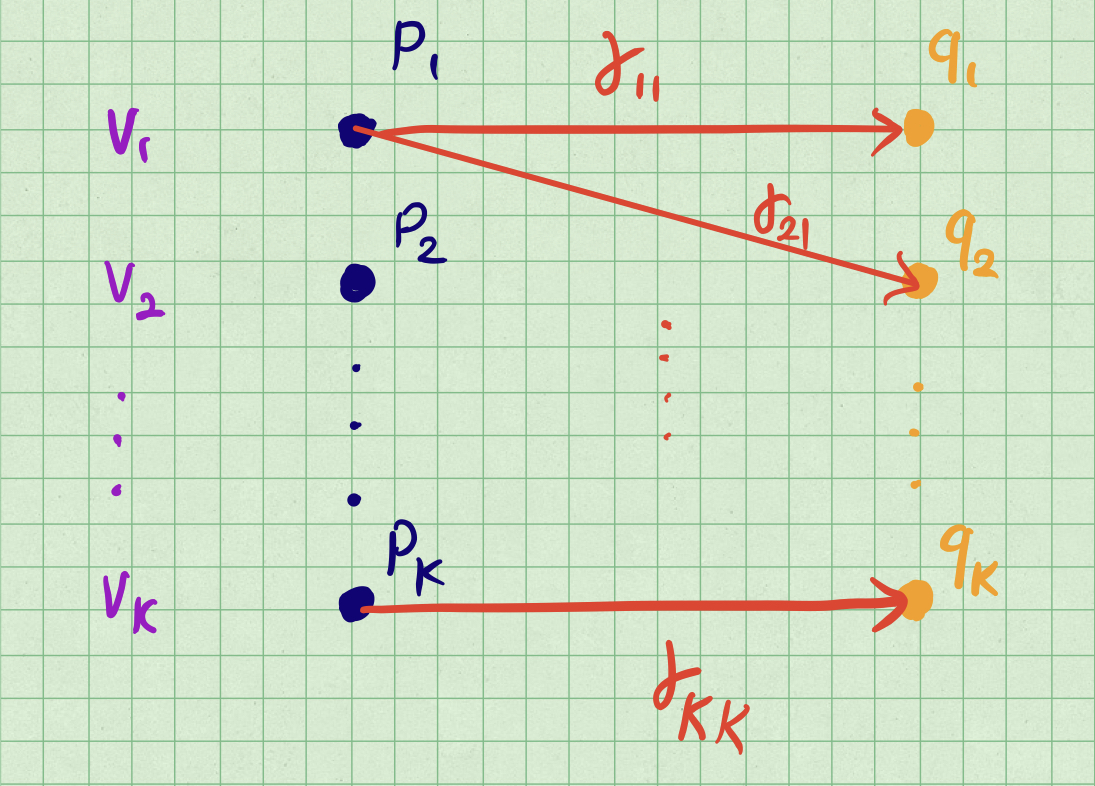
\includegraphics[width=0.6\textwidth]{gammaDiag.jpg}
     \caption{Diagram representation of coupling}
     \label{fig:coupling}
\end{figure}
\\
Last lecture, we shortly discussed why other distance measures ($e.g.$, Total Variation (TV) distance and Kullback-Leibler(KL) divergence) are not useful in our setting compared to Wasserstein distance. Before we move on to the formal proof of Theorem 1, here we discuss and compare Wasserstein distance with TV distance and KL divergence.\\
\\
\textbf{Definition 3} (Total Variation distance).
\begin{align*}
    \text{TV}(P,Q) &= \underset{0 \le f \le 1}{\sup} \hspace{0.25em}
                     \abs{ \bbE_{x \sim P} \left[ f(x) \right] -
                     \bbE_{x \sim \mathcal{Q}} \left[ f(x) \right]}
  &(\textit{All cases})\\
    &= \frac{1}{2} \int \abs{p(x) - q(x)} dx \quad \text{where $P$ and $Q$ have densities $p$ and $q$} &(\textit{Continuous case})
\end{align*}
\\
\textbf{Definition 4} (Kullback-Leibler divergence).
\begin{align*}
    \text{KL}(P,Q) &= \bbE_{x \sim P} \left[\log \frac{p(x)}{q(x)} \right] = \sum_x P(x) \log \frac{P(x)}{Q(x)} &(\textit{Discrete case})\\
    &= \int_{-\infty}^\infty p(x) \log \left( \frac{p(x)}{q(x)} \right) dx &(\textit{Continuous case})
\end{align*}
\\
\noindent \textbf{Example 1.} Suppose $P$ is uniform distribution over sphere and $Q$ is also uniform distribution over sphere which is shifted by $\epsilon$ on only one coordinate. Let the metric $d = l_2$. Figure~\ref{fig:sphere} shows two distributions of $P$ and $Q$.\\
    \begin{figure}[h]
  \centering
    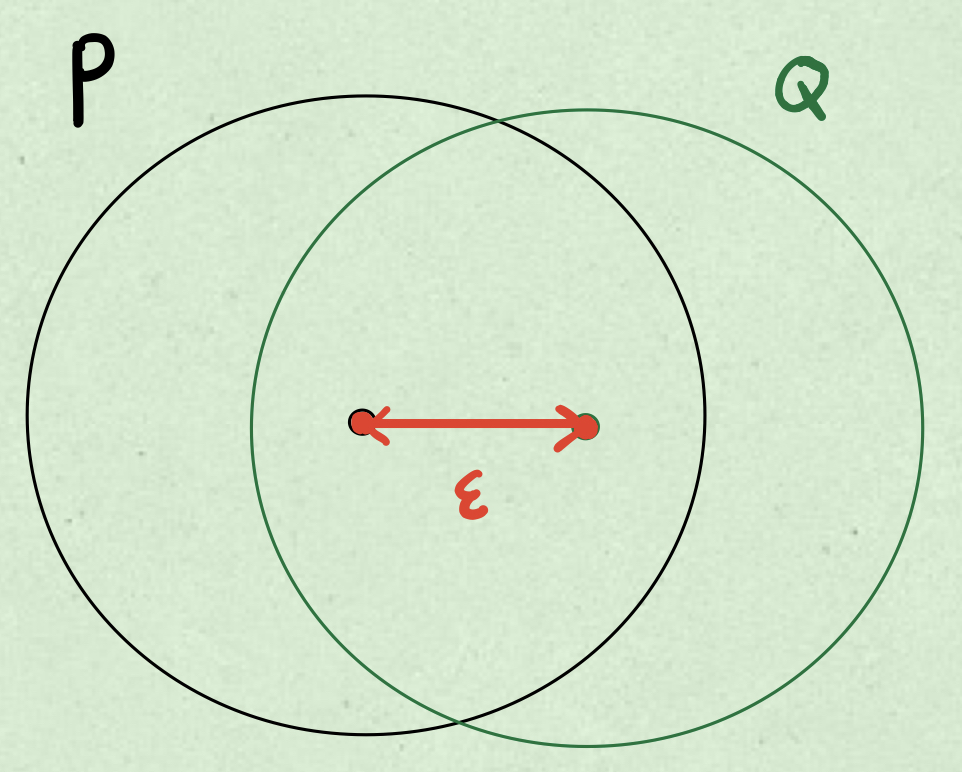
\includegraphics[width=0.3\textwidth]{sphere.jpeg}
     \caption{Distributions of $P$ and $Q$}
     \label{fig:sphere}
\end{figure}
\\
\noindent  In this case, TV$(P,Q) = 1$ because we can construct the function $f$ as following:
\begin{align*}
    f(x) &= 1 \quad \text{if} \quad X \in \text{support}(P)\\
    f(x) &= 0 \quad \text{if} \quad X \in \text{support}(Q)
\end{align*}
Note that KL$(P,Q)$ is not well-defined in this setting because not both $P$ and $Q$ defined on the same probability space. On the other hand, $W_1(P,Q) \le \epsilon$. To see why this is the case, we first construct a coupling as following sampling technique:
\begin{align*}
    (x,y) \sim \mathcal{P} \quad \Longleftrightarrow \quad x \sim P, y = x + \epsilon \begin{bmatrix}
    1\\
    0
    \end{bmatrix}
\end{align*}
Note that the marginal distribution would  be $P$ and $Q$. Here, we achieve 
\begin{align*}
    W_1(P,Q) &= \bbE_{(x,y) \sim \mathcal{P}} \left[d(x,y) \right] \\
    &= \bbE_{(x,y) \sim \mathcal{P}} \left[ \norm{x-y}_2 \right] \\
    &= \epsilon  &\text{since } x-y = \epsilon \cdot \begin{bmatrix}
    1 \\
    0
    \end{bmatrix}
\end{align*}
\noindent \textbf{Example 2.} We state the following claim:\\
\\
\textbf{Claim 1.} TV$(P,Q) = W_1(P,Q)$ with respect to the trivial metric $d(x,y) = \1 \left\{ x \neq y \right\}$ \\
(Note: This claim explains why TV distance does not take into account geometry.) \\
\\
\textit{Proof.} $f$ is 1-Lipschitz with respect to the metric $d(x,y) = \1 \left\{ x \neq y \right\}$. We claim that
\begin{align*}
    \abs{f(x) - f(y)} \le \1 \left\{ x \neq y \right\} \quad \Longleftrightarrow \quad \underset{x \in \mathcal{X}}{\sup} \hspace{0.5em} f(x) - \inf(f) \le 1
\end{align*}
To see this, first note that from $|f(x)-f(y)|\le I\{x\ne y\}$, we get that $|f(x)-f(y)|\le 1$ if $x\ne y$. Thus, if the elements obtaining the sup and inf are not the same, then the difference is bounded by 1, otherwise the difference will be 0. Furthermore, if $\sup_{x \in \mathcal{X}} f(x)- \inf(f) \le 1$, it immediately follows that $|f(x) - f(y)| \le 1 \ \forall x, y$. This establishes the equivalence.

From here, we denote $\bbE_{x \sim P} \left[ f(x) \right] =\bbE_{x \sim P} f $ and $\bbE_{x \sim Q} \left[ f(x) \right] =\bbE_{x \sim Q} f $ for simplicity. Then,
\begin{align*}
    W_1(P,Q) &= \underset{f: \sup f - \inf f \le 1}{\sup} \underbrace{\bbE_{x \sim P} f - \bbE_{x \sim Q} f}_{\text{shift invariant}} \\
    &= \underset{f: 0 \le f \le 1}{\sup} \bbE_{x \sim P}f - \bbE_{x \sim Q}f \\
    &= \underset{\substack{{f: 0 \le f \le 1,}\\ {0 \le 1-f \le 1}}}{\max} \left\{ \bbE_{x \sim P} f - \bbE_{x \sim Q} f, \quad \bbE_{x \sim P} (1-f) - \bbE_{x \sim Q} (1-f)  \right\} \\
    &= \underset{0 \le f \le 1}{\sup} \abs{\bbE_{x \sim P} f - \bbE_{x \sim Q} f} \\
    &= TV(P,Q)
\end{align*}

\noindent where the second equality follows from the fact that $\bbE_{x \sim P} f - \bbE_{x \sim Q} f$ is shift invariant ($i.e.$, $\bbE_P [f + c] - \bbE_Q [f + c] = \bbE_P f + c - \bbE_Q f - c = \bbE_P f - \bbE_Q f),$ and thus we can subtract $\inf f$. The fourth equality is again using the fact that $\bbE_{x \sim P} (1-f) - \bbE_{x \sim Q} (1-f)$ is shift invariant and thus we can remove $1$ and have the second term become $\bbE_P(-f) - \bbE_Q(-f)$.

\subsection{Proof of Kontorovich-Rubinstein duality}
We use LP duality in fuctional space with $f$ as variable to prove \textbf{Theorem 1}. \\
\\
Assume $\mathcal{X}$ is finite: $\mathcal{X} = \{v_1, ..., v_k\}$ and $f(v_1),...,f(v_k) \triangleq (f_1,...,f_k)$ and recall that $P = (p_1,...,p_k), Q = (q_1,...,q_k)$. As usual, we assume $p_i > 0, q_i > 0$ for all $i$. We construct the following linear programming problems:
\begin{itemize}
    \item \textbf{Program (A)}:
    \begin{align*}
        \mbox{$\underset{f = (f_1,...,f_k)}{\text{maximize}}$} \quad &\sum_{i=1}^k p_if_i - \sum_{i=1}^k q_if_i &\left(\text{OPT}_1\right)\\
        \mbox{subject to} \quad &f(x) - f(y) \le d(x,y) \quad \forall x,y \in \mathcal{X}\\
        &(\text{$i.e.$, } f(v_i) - f(v_j) \le d(v_i, v_j) \Longleftrightarrow f_i - f_j \le d_{ij})
    \end{align*}
    Note that OPT$_1$ is the expanded version of the objective function: $\underset{f}{\max}$ $\bbE_P f - \bbE_Q f$.
    \item \textbf{Program (P)}:
    \begin{align*}
        \mbox{$\underset{\gamma}{\text{minimize}}$} \quad &\sum_{i,j} \gamma_{ij} d_{ij} &\left(\text{OPT}_2\right)\\
        \mbox{subject to} \quad &\sum_j \gamma_{ij} = p_i \quad \forall i &\left(\text{dual: } \textcolor{red}{f_i} \right)\\
        &\sum_i \gamma_{ij} = q_j \quad \forall j &\left(\text{dual: } \textcolor{red}{-g_j} \right)\\
        &\gamma_{ij} \ge 0 \quad \forall i,j &\left(\text{dual: } \textcolor{red}{w_{ij}} \right)
    \end{align*}
\end{itemize}

\noindent \textbf{Goal.} We want to prove that OPT$_1$ = OPT$_2$. \\
\\
\noindent \textbf{Lemma 1} (OPT$_1$ $\le$ OPT$_2$).\\
\textit{Proof.} Let $f, \gamma$ be optimal solutions to \textbf{(A)} and \textbf{(P)} respectively. Then,
\begin{align*}
    \text{OPT}_1 &= \sum_i (p_i - q_i) f_i\\
    &= \sum_i (\sum_j \gamma_{ij}) f_i - \sum_i(\sum_j \gamma_{ji}) f_i &\left(\text{by definition of $p_i$ and $q_i$}\right)\\
    &= \sum_i (\sum_j \gamma_{ij}) f_i - \sum_j(\sum_i \gamma_{ij}) f_j\\
    &= \sum_{i,j} \gamma_{ij}(f_i - f_j) \\
    &\le \sum_{i,j} \gamma_{ij} d_{ij} = \text{OPT}_2.
\end{align*}

\noindent Next, we construct the dual of \textbf{(P)} using dual variables specified in parentheses in \textbf{(P)}:
\begin{itemize}
    \item \textbf{Program (D)}:
    \begin{align*}
        \mbox{$\underset{f,g}{\text{maximize}}$} \quad &\sum_i p_if_i - \sum_i q_ig_i &\left(\text{OPT}_3\right)\\
        \mbox{subject to} \quad & f_i - g_j + w_{ij} = d_{ij} \quad \forall i,j
    \end{align*}
    Note that the constraint can be re-written as $f_i - g_j \le d_{ij} \quad  \forall i,j$ because $w_{ij}$ is nonnegative by definition of dual variable.\\
\end{itemize}

\noindent \textbf{Lemma 2} (OPT$_1$ $\ge$ OPT$_3$).\\
\textit{Proof.} The main idea here is to use the fact that $d$ is a metric. Let $f, g, \gamma$ be optimal solutions to \textbf{(P)} and \textbf{(D)}. Then, by \emph{complementary slackness}\footnote{If you are not familiar with this part, please refer to Chapter 5 of \emph{Convex Optimization}~\cite{BoV:04} and/or EE 364A course lecture slide 17 on \url{http://web.stanford.edu/class/ee364a/lectures/duality.pdf}},
$$f_i - g_j = d_{ij} \quad \text{if} \quad \gamma_{ij} > 0 \quad \forall i,j.$$
First, we show that $g_j - g_t \le d_{jt} \quad \forall j,t$ by following
\begin{align*}
    \forall j, \text{ pick } i \text{ such that } \gamma_{ij} > 0 \quad &\Longrightarrow \quad f_i - g_j = d_{ij} & (1)\\
    \text{ Also, by constraint: } &\forall i,t \quad f_i - g_t \le d_{it} & (2)
\end{align*}
$(1) - (2)$ yields: $g_j - g_t \le d_{it} - d_{ij} \le d_{jt}$ where the last inequality is from triangle inequality as $d$ is a metric. Therefore, $g$ is a feasible solution of \textbf{(A)}. Note that from \textbf{(D)}'s constraint, $f_i - g_i \le d_{ii}$ and $d_{ii} = 0$ since it's a metric. Therefore, $f_i \le g_i$ for all $i$. Using this, we obtain:
\begin{align*}
    \text{OPT}_1 &\ge \sum_i p_ig_i - \sum_i q_ig_i &\left( \text{feasibility of } g\right)\\
    &\ge \sum_i p_if_i - \sum_i q_ig_i &\left( f_i \le g_i\right)\\
    &= \text{OPT}_3.
\end{align*}

\noindent Finally, by \textbf{Lemma 1} and \textbf{Lemma 2} and the fact that OPT$_2$ = OPT$_3$\footnote{Since OPT$_3$ is dual of OPT$_2$ and \emph{strong duality} holds for linear programming, OPT$_2$ = OPT$_3$.}, we conclude
$$\text{OPT}_1 = \text{OPT}_2 = \text{OPT}_3.$$

\section{Plans for future lectures}
Recall that the main question we aim to address is:\\
\begin{itemize}
\item[] $\quad
    \underbrace{W_\mathcal{F} (\hat p, \hat p_\theta )}_{\text{training loss}} \quad \text{small} \quad  \Longrightarrow \quad W_1 \left( p, p_\theta \right) \quad \text{small}$ \textcolor{red}{ ? } \\
\end{itemize}
Our plan for addressing this question is following:
\begin{itemize}
\item[] \emph{Plan}: $\quad
W_\mathcal{F} (\hat p, \hat p_\theta ) \quad \xleftrightarrow{\text{generalization}} \quad W_\mathcal{F} (p,p_\theta) \quad \xleftrightarrow{\text{approx.} W_1 \approx W_\mathcal{F}} \quad W_1(p,p_\theta).$\\
\end{itemize}
\noindent Hence, in the next lecture we will show three observations:
\begin{enumerate}
    \item If $\mathcal{F}$ is complex $\Longrightarrow$ generalization is \textbf{bad}
    \item If $\mathcal{F}$ has small complexity $\Longrightarrow$ generalization is \textbf{good}
    \item If $\mathcal{F}$ has small complexity $\Longrightarrow$ approximation \textbf{may not be good}
\end{enumerate}
and explore ways to overcome this dilemma.

\bibliography{10_29_final}

%%% Scribe due date: 10/31 11PM

%%%%%%%%%%%%%%%%%%%%%%%%%%%%%%%%%%%%%%%%%%%%%%%%%%%%%%%%%%%%%%%%

\end{document}